\chapter{RL for {\sc ltl}$_f$/{\sc ldl}$_f$ Goals}\label{ch:rl-llf-goals}

In this chapter, we describe one of the main contributions of the thesis. We define a particular problem, that we call
\emph{Reinforcement Learning for \LLf Goals}, and propose a solution.
We focus on the case where we have two separate representations of the world: one for the agent, using the \emph{low-level} features available to it, and one for the goal, expressed in terms of \emph{high-level} (human-understandable) fluents.

In the first section, we describe the context of the problem and the motivations, whereas in the second section we give a formal definition. In the next section, we show how we can reduce this problem to do reinforcement learning on an equivalent MDP. Finally, we give an episodic view of the scenario, which is the one used in the implementation of the experiments.

\section{Introduction and Motivations}
Let consider to have a
learning agent equipped with sensing procedures to compute
a set of features from the world that forms its states and with
a set of actions that it can do. 
For example, you can imagine a robot in a room that can move in many directions; its state space can be a combination of features measured from different physical quantities e.g. its position in the room.

Our purpose in this work is to use this agent
to learn one (or simultaneously many) task whose goal (or many goals)
are expressed in \LLf. Such goals are expressed over
a representation of the world that is not the one used by the
agent (oversimplifying, we may say that the agent has a low-level representation), but a convenient high-level representation suitable to express declaratively temporally extended goals. In other words, we study the possibility of having \emph{two
separate representations of the world}:
\begin{itemize}
	\item one for expressing the dynamics of the RL agent;
	\item one for expressing the \LLf goals.
\end{itemize}

These two representations use different classes of features
from the real world: the first includes the features that the agent can directly access, while the second includes the features needed to evaluate the \LLf goal.

One may ask: why we need two \emph{separated} representation of the world? Why can we not merge them into a unique representation and reason/learn over this joint model?

There are many reasons why this might be useful:
\begin{enumerate}
	\item The agent feature space can be designed separately from
	the features needed to express the goal, thus promoting
	\emph{separation of concerns} which, in turn, facilitates the design; this separation facilitates also the \emph{reuse} of representations already available, possibility developed for the standard setting.\label{motivation:separation-of-concern}
	
	\item A reduced agent's feature space allows for realizing \emph{simpler agents} while preserving the possibly of tackling complex declarative goals which cannot be represented in the agent's feature space. \label{motivation:simpler-agent}
	
	\item Reducing the agent's feature space may yield a \emph{reduced} state space to be explored by the RL-agent.\label{motivation:reduced-space}
	
\end{enumerate}

Clearly, the two separate representations (i.e., the two sets
of features) need to be somehow correlated in reality. The crucial point, however, is that in order to perform RL effectively, \emph{such a correlation does not need to be formalized}. We let the reinforcement learning agent learn, over its state space (eventually extended), the proper way to use an arbitrary long sequence of low-level actions in order to accomplish the high-level goals.

\begin{example}
	Consider the RL environment \Breakout (Example \ref{exa:breakout}). Let the agent's state space be the combination of the paddle position, the ball position and the ball speed. The actions available to the agent are: move to the left, move to the right, and a nop-action. The goal is to remove all the bricks by hitting and directing the ball in a proper way.
	
	Now suppose that we want to express a \LLf goal, which is a sort refinement of the agent's goal: to break columns of bricks in a precise order (e.g. from left to right). To express this goal we need:
	\begin{itemize}
		\item a set of features that allow detecting the status of the bricks;
		\item a mapping of those features to a set of fluents upon which the \LLf formula can be expressed (e.g. the status of each column of bricks).
	\end{itemize}
	In this case, the agent's state space represents the \emph{low-level} state space, whereas all the possible configurations of the fluents represent the \emph{high-level} state space.
	
	Notice that for the satisfaction of the \LLf goal defined above, we don't need to include every possible configuration of the fluents (i.e. status of every brick) into the state space of the learning agent; instead, our intuition suggests that the RL agent, in order to be able to learn the optimal action in a given state, \emph{needs only to keep track at which point of the satisfaction of the goal it is}, such that it is able to learn how to proceed, until the complete satisfaction of the goal.
	
	In our example, the learning agent just needs to know which is the next column of bricks to remove. Hence, besides the agent's state space, the agent needs to know the current target column, up to $n$ different sub-goals, where $n$ is the number of columns. In this way, it can learn how to break the current target column, and inherently the sequence of actions that lead to the removing of every column, one by one, in sequence.
	
	Another question may arise: why one should need the proposed construction (i.e. the extended state space for temporal goals from the  \LLf specification) instead of a state space composed by ad-hoc features set for specifying the desired temporal goal?
	
	The last considerations and the following ones should convince the reader about the main advantages of our approach:
	\begin{itemize} 
		\item \emph{Reduced state space} (motivation \ref{motivation:reduced-space}). Let $\States$ be the agent's state space. The minimum size of the learning state space needed to the agent is $|\States| \cdot n$, where the $n$-fold increase of $\States$  allow to discern a state $s\in\States$ in different partial satisfaction of the goal (i.e. the last column removed). Hence, we do not need to include directly the status of each brick, which would return a feature space of size $|\States| \cdot 2^{mn}$ ($n$ i the number of columns of bricks and $m$ is the number of rows). Notice that the latter state space is \emph{exponentially} bigger than the minimal one, which is only linear in the number of columns. 
		\item \emph{Easier feature design} (motivation \ref{motivation:separation-of-concern}). Even if, with traditional feature engineering, it is possible to build a composed state space that includes the needed pieces of information for learning temporally extended goal, the result is a hard-coded model, rigid to modifications. On the other hand, our approach is more flexible and open to modifications, both on features/fluents level and on \LLf goal level (just add/modify \LLf formulas).
		\item \emph{Declarativeness}: specifying by hand how the state components that track the temporal goal should evolve could be very hard and unintuitive. Instead, \LLf formalisms allow to easily express a wide range of temporal goals about how fluents should change over time.
	\end{itemize}
	
\end{example}

\medskip

How the learning state space (i.e. the state space over where the agent actually learns) can be deduced by the \LLf formula and the fluents configuration is the topic of the following sections.

In order to proceed with a formal definition of the problem, we made the following working assumption:
\begin{itemize}
	\item The agent's model of the world is an MDP; in particular, the transitions from a state to another state, given an action, satisfies the Markov property;
	\item The granularity of the state representations is enough to accomplish the \LLf goals. It might be the case that the high-level or the low-level representation of the world is somehow inadequate to capture the relevant changes in the world;
	\item Notice that, in our setting, from the agent's point of view, the changes of the agent's state space and the ones of the fluents are \emph{synchronous}, and depends from a \emph{clock}, implicit in the model definition. Hence, we assume that this synchrony, as well as the granularity resulting from the clock, still allow the agent to learn to properly optimize the rewards.
\end{itemize}


\section{Problem definition}
\label{sect:problem-definition}
In this section, we describe more formally the scenario. We first give an overall picture of the model. then, we make an important observation about the transition function of the joint world representations. Finally, we define the mathematical model that will be used in the next section.
\subsection{The World, the Agent and the Fluents}
Let $\W$ be a \emph{world} of interest (e.g. a room, an environment, a video game). Let $W$ be the set of \emph{world states}, i.e. the states of the world $\W$. 
A \emph{feature} is a function $f_j$ that maps a world state to the
values of another domain $D_j$, such as reals, finite enumerations,
booleans, etc., i.e., $f_j : W \rightarrow D_j$.
%%
Given a set of features $F = \tup{f_1, \dots, f_d}$, the \emph{feature vector} of a world state $w_h$ is the vector
$\mathbf{f}(w_h) = \langle f_1(w_h), \ldots, f_d(w_h) \rangle$ of
feature values corresponding to $w_h$.
%%

Now consider an agent that lives in $\W$. The agent can interact with $\W$ by executing an action $a$ taken from a \emph{set of actions} $\Actions$. Without loss of generality, we assume that such a learning agent has a special action $\Stop$ which deems the end of an episode.
Moreover, the agent has its own set of features $F_{ag} = \tup{f_1, \dots, f_d}$, which yields its \emph{representation of the world} $\States$, where $\States \subseteq F_{ag}(W)$ and $F_{ag}(W) = \set{\mathbf{f}_{ag}(w) | w \in W}$. We assume that the agent has a \emph{clock} which determines the granularity of its acting. At every clock, the agent can do action $a$ and observe both the new state $s$ from the new world state $w'$, namely $s = \mathbf{f}_{ag}(w)$, and a real-valued reward $R(s,a,s')$, that depends only from the transition $s\to_a s'$.
Finally, we assume that the law that determines the possible next state $s'$ given the history of a trajectory (i.e. the state transition function $\TrFun$) is Markovian, hence it depends only from the current state $s$ and the taken action $a$. 
In other words, we can define an MDP $\MDPagent = \tup{\States, \Actions, \TrFun, \Reward, \DiscFact}$.

We consider arbitrarily \LLf formulas $\varphi_i$
($i=1,\ldots,m$) over a set of fluents $\F$ used to provide a high-level description of the world. We denote by $\L=2^\F$ the set of possible fluents configurations. 
Given a set of features $F_{goal}$, a \emph{configuration of fluents} $\ell_h \in \L$ is formed by the components that assign truth values to the fluents according to
the feature vector $\mathbf{f}_{goal}(w_h)$. At every step, the features for fluents evaluations are observed, obtaining a particular configuration $\ell\in\L$. Notice that in general the features for the fluents and for the agent state space may differ. The formula $\varphi_i$ is
selecting sequences of fluents configurations $\ell_1,\cdots,\ell_n$,
with $\ell_k\in \L$, whose relationship with the sequences of states
$s_1,\ldots, s_n$, with $s_k \in S$ is unknown.

 In other words, a subset of features are used to describe agent states $s_h$ and another  subset (for simplicity, assumed disjoint from the previous one) are used to evaluate the fluents in $\ell_h$.
 %%
 Hence, given a sequence $w_1,\ldots,w_n$ of
 world states we get the corresponding sequence of sequences learning
 agent states $s_1,\ldots,s_n$ and simultaneously the sequence of fluent
 configurations $\ell_1,\ldots,\ell_n$.  Notice that we do not have a
 formalization for $w_1,\ldots,w_n$ but we do have that for $s_1,\ldots,s_n$
 and for $\ell_1,\ldots,\ell_n$. 


Oversimplifying, we may say that $S$ is the set of configurations of
the low-level features for the learning agent, while $\L$ is
the set of configuration of the high-level features needed for
expressing $\varphi_i$.

Figure \ref{fig:rl-schema} depicts the above described scenario. You can recognize how the world state $w$ contributes both to the generation of the agent's state $s$ and of the fluents configurations $\ell$.

\begin{figure}[h]
	\centering
	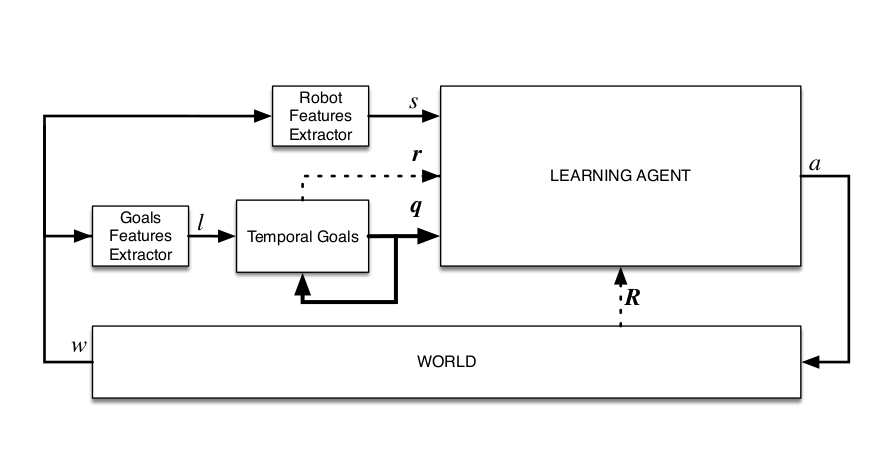
\includegraphics[width=\textwidth]{images/rl-two-representations}
	\caption{The reinforcement learning system for temporally extended goals.}\label{fig:rl-schema}
\end{figure}

\subsection{Joint transition function}
Now we consider the transition distribution over the features, the agent actions in $A$ and the fluents configuration, i.e.,
\begin{equation}\label{joint-tr-fun}
\TrFun_{ag}^{g} : S\times \L \times A \rightarrow Prob(S\times \L)
\end{equation}
We observe that the state transition function $\TrFunAgentGoal$ is \emph{Markovian}, i.e. the probability to end in the next state $s'$ with the next fluents configuration $\ell'$ depends only from $s, \ell$ and $a$ (the current agent state, the current fluents configuration and the action taken, respectively).

Actually, the observation is necessary, under the assumption that the evolution of the agent's state space component is Markovian. Indeed, it might happen that the introduction of the fluents configurations in the transition model violates the Markov property of the transition function in Equation \ref{joint-tr-fun}; however, we notice that, if this is the case, we can expand $\L$ by including many other fluents, as much as it is needed to make the transition function Markovian.

We will see that this mathematical trick does not affect the following results, because $\L$, at the end of the day, \emph{does not matter to the learning agent}.
So, without loss of generality, we consider the joint transition function in Equation \ref{joint-tr-fun} is Markovian, even if the considered set of fluents configurations $\L$ makes the transition function to violates the Markov property for some transitions.

Such a transition distribution together with the initial values of the
fluents $\ell_0$ and of the agent state $s_0$ allow us to describe a
probabilistic transition system accounting for the dynamics of the
fluents and agent states. 
In other words, in response to an agent action $a_h$ performed in the current state
$w_h$ (in the state $s_h$ of the agent and the
configuration $\ell_h$ of the fluents), the world changes into $w_{h+1}$ from which $s_{h+1} $ and $\ell_{h+1}$. This is all we need to proceed.

\medskip

\subsection{Formal definition}
We are interested in devising policies for the learning agent such that
at the end of the episode, i.e., when the agent executes \emph{stop},
the \LTLf /\LDLf goal formulas $\varphi_i$ ($i=1,\ldots,m$)  are satisfied.
%%
Now we can state our problem formally.

\noindent
\begin{definition}\label{def:rl-for-llf-goals}
	 \textit{
	We define \emph{RL for \LTLf /\LDLf goals}, denoted as
	\[\MDPagent^{goal}= \tup{\States, \Actions, \Reward, \L, \TrFunAgentGoal, \{(\varphi_i,r_i)\}_{i=1}^{m}}\] with $\TrFunAgentGoal$, $\Reward$ and
	$r_i$ unknown,the following problem: given a learning agent
	$\MDPagent = \tup{\States, \Actions, \TrFun, \Reward}$, with $\TrFun$ and $\Reward$ unknown and
	a set $\{(\varphi_i,r_i)\}_{i=1}^{m}$ of \LTLf /\LDLf formulas with
	associated rewards, find a (non-Markovian) policy
	$\NMPolicy:\States^*\rightarrow A$ that is optimal wrt the sum of the rewards
	$r_i$ and $\Reward$.}
\end{definition}
Observe that an optimal policy for our problem, although not depending on $\L$, is guaranteed to satisfy the \LTLf /\LDLf goal formulas.


\section{Reduction to MDP}\label{sect:rl-goals-reduction-to-mdp}
To devise a solution technique, we start by transforming
$\MDPagent^{goal}= \tup{\States, \Actions, \TrFunAgentGoal, \Reward, \L,
\{(\varphi_i,r_i)\}_{i=1}^{m}}$ into an NMRDP $\MDPagent^{nmr} = \langle S\times \L, A, \TrFunAgentGoal, \{(\varphi'_i,r_i)\}_{i=1}^{m} \cup \{(\varphi_s, R(s,a, s'))\}_{s\in S, a\in
	A, s'\in S} \rangle$ where:
\begin{itemize}
	\item States are pairs $(s,\ell)$  formed by an agent configuration $s$ and a fluents configuration $\ell$.
	\item $\varphi'_i = \varphi_i \land \Diamond Done$.
	\item $\varphi_s = \Diamond(s\land a\land \Next(\Last \land s'))$.
	\item $\TrFun_{ag}^{g}$, $r_i$ and  $R(s,a, s')$ are unknown and sampled from the environment.
\end{itemize} 

Formulas $\varphi'_i$ simply require to evaluate the corresponding
goal formula $\varphi_i$ after having done the action $stop$, which
sets the fluent $Done$ to true and ends the episode. Hence it gives
the reward associated with the goal at the end of the episode.
%%
The formulas $\Diamond(s\land a\land \Next(Last \land s'))$, one per
$(s,a,s')$, requires both states $s$ and action $a$ are followed by
$s'$ are evaluated at the end of the current (partial) trace (notice
the use of $Last$).  In this case, the reward $R(s,a,s')$ from
$\MDPagent$ associated with $ (s,a,s')$ is given.  


Notice that policies for $\MDPagent^{nmr}$ have the form
$(S\times\L)^*\rightarrow A$ which needs to be restricted to have the form required by our problem
$\MDPagent^{goal}$.



A policy $\NMPolicy:(\States\times\L)^*\rightarrow A$ \emph{has the form} $\States^*\rightarrow \Actions$
when for any sequence of $n$ states
$\langle s_1 \cdots s_n\rangle$,
we have that 
for any pair of sequences of fluent configurations 
$\langle \ell'_1 \cdots \ell'_n\rangle$, 
$\langle \ell''_1 \cdots \ell''_n\rangle$
the policy returns the same action, 
$\NMPolicy(\langle s_1,\ell'_1\rangle \cdots \langle s_n,\ell'_n\rangle) = \NMPolicy(\langle s_1,\ell''_1\rangle \cdots \langle s_n,\ell''_n\rangle)$.
%%
In other words, a policy  $\NMPolicy:(S\times\L)^*\rightarrow A$ has the form $\NMPolicy:S^*\rightarrow A$ when it does not depend on the fluents $\L$. 
%%
We can now state the following result.


\begin{theorem}\label{th:goal-nmr}
	RL for \LTLf /\LDLf goals
	$\MDPagent^{goal}= \langle S, A, Tr^{g}_{ag}, R, \L,
	\{(\varphi_i,r_i)\}_{i=1}^{m}\rangle$ can be reduced to RL over the
	NRMDP
	$\MDPagent^{nmr} = \langle S\times \L, A, \TrFun_{ag}^{g},
	\{(\varphi'_i,r_i)\}_{i=1}^{m}\cup \{(\varphi_s, R(s,a, s'))\}_{s\in S,
		a\in A, s'\in S} \rangle$, 
	%     restricting policies  to be learned to have the form such that  the restriction on $S^*$ of the optimal policy for  $\MDPagent^{nmr}$ is an optimal policy
	% for $\MDPagent^{goal}$.    
	restricting policies to be learned to have the form $S^*\rightarrow A$.
\end{theorem}

Observe that by restricting $\MDPagent^{nmr}$ policies to $S^*$, in general, we may discard policies that have a better reward but depend on $\L$. On the other hand, these policies need to change the learning agent in order to allow it to observe $\L$ as well. As mentioned in the introduction, we are interested in keeping the learning agent as it is, apart from additional memory.

\medskip
As a second step, we apply the construction of Section \ref{sect:nmrdp-llf-rewards} and obtain a
new MDP learning agent.  In such construction, however, because of the
triviality of their automata, we do not need to keep track of state
$\varphi_s$, but just give the reward $R(s,a,s')$ associated to
$(s,a,s')$. Instead, we do need to keep track of the state of the \DFAs
$\automaton_{\varphi_i}$ corresponding to the formulas $\varphi'_i$.
Hence, from $\MDPagent^{nmr}$, we get an MDP $\MDPagent'=\langle S',A',Tr'_{ag},R'\rangle$ where:
\begin{itemize}\itemsep=0mm
	\item $S'=Q_1\times\cdots\times Q_m\times S\times \L$ is the set of states;
	\item $\Tr'_{ag} : S'\times A' \times S'\rightarrow [0,1]$ is defined as follows:
	\[
	\begin{array}{l}
	Tr'_{ag}(q_1,\ldots,q_m, s,\ell, a, q'_1,\ldots,q'_m, s',\ell') = {}\\
	\quad\left\{
	\begin{array}{ll}
	Tr(s,\ell,,a,s',\ell') &\mbox{if } \forall i:\delta_i(q_i,\ell') = q'_i\\
	0 & \mbox{otherwise}; 
	\end{array}\right.
	\end{array}
	\] 
	\item $R': S'\times A \times S' \rightarrow 
	\mathbb{R}$ is defined as:
	\[\begin{array}{l}
	R'(q_1,\ldots,q_m, s,\ell, a, q'_1,\ldots,q'_m, s',\ell') = {}\\
	\qquad
	\sum_{i: q'_i\in F_i} r_i+R(s,a,s')
	\end{array}
	\] 
\end{itemize}
Finally we observe that the environment gives now both the rewards $R(s,a,s')$ of the original learning agent, and the rewards $r_i$ associated to the formula so has to guide the agent towards the satisfaction of the goal (progressing correctly the \DFAs $\automaton_{\varphi_i}$).

By applying Theorem~\ref{th:nmrdp-mdp-llf-equivalence} we get that NMRDP $\MDPagent^{nmr}$ and
the MDP $\MDPagent'$ are equivalent, i.e., any policy of $\MDPagent^{nmr}$
has an equivalent policy (hence guaranteeing the same reward) in
$\MDPagent'$ and vice versa. Hence we can learn policy on $\MDPagent'$ instead of $\MDPagent^{nmr}$. 
%%

We can refine Theorem~\ref{th:goal-nmr} into the following one.

\begin{theorem}\label{th:goal-mdp-ell}
	RL for \LTLf /\LDLf goals
	$\MDPagent^{goal}= \tup{\States, \Actions, \TrFunAgentGoal, \Reward, \L,
	\{(\varphi_i,r_i)\}_{i=1}^{m}}$ can be reduced to RL over the
	MDP $\MDPagent'=\tup{\States',\Actions,\TrFun'_{ag},\Reward'}$,
	restricting policies to be learned to have the form $Q_1\times\ldots\times Q_n\times S\rightarrow A$. %
	%    such that  the restriction on $Q_1\times\ldots\times Q_n\times S$ (i.e, projecting out $\L$) of the optimal policy for  $\MDPagent^{nmr}$ is an optimal policy
	% for $\MDPagent^{goal}$. 
	%   and the optimal policy $\Policy_{ag}'$ learned for $\MDPagent'$ can be reduced to a corresponding optimal policy for $\MDPagent^{goal}$ restricted to policies to be learned to have the form $\Policy:S^*\rightarrow A$.
\end{theorem}
As before, a policy $Q_1\times\ldots\times Q_n\times S \times \L \rightarrow \Actions$ \emph{has the
	form} $Q_1\times\ldots\times Q_n\times S\rightarrow A$ when any
$\ell$ and $\ell'$ the policy returns the same action,
$\Policy(q_1,\ldots, q_n s,\ell) = \Policy(q_1,\ldots, q_n s,\ell') $.


\medskip
The final step is to
%In practice we can 
solve our original RL task on $\MDPagent^{goal}$ by performing RL on a new MDP 
$\MDPagent^{new}=\langle Q_1\times\cdots\times Q_m \times S,A,\TrFun''_{ag},R''\rangle$ where:
\begin{itemize}
	\item  Transitions distribution $\TrFun''_{ag}$ is the marginalization wrt $\L$ of $\TrFun'_{ag}$ and is unknown;
	\item  Rewards $R''$ is defined as:
	\[
	R''(q_1,\ldots,q_m, s, a, q'_1,\ldots,q'_m, s') = \sum_{i: q'_i\in F_i} r_i+R(s,a,s').
	\] 
	\item States $q_i$ of \DFAs $\automaton_{\varphi_i}$ are progressed correctly by the environment.
\end{itemize}

Indeed, we can show the following result.

\begin{theorem}\label{th:goal-mdp}
	RL for \LTLf /\LDLf goals
	$\MDPagent^{goal}= \tup{\States, \Actions, \TrFun', \Reward, \L,
	\{(\varphi_i,r_i)\}_{i=1}^{m}}$ can be reduced to RL over the
	MDP $\MDPagent^{new}=\tup{Q_1\times\cdots\times Q_m \times \States, \Actions,\TrFun''_{ag},\Reward''}$
	and the optimal policy $\Policy_{ag}^{new}$ learned for $\MDPagent^{new}$ can be reduced to a corresponding optimal policy for $\MDPagent^{goal}$. 
\end{theorem}

\begin{proof}
	From  Theorem~\ref{th:goal-mdp-ell}, by the following observations. For the sake of brevity, we use $\bqs$ to denote $q_1, \dots, q_m$.
	Notice also that for all $\ell, \ell'\in\L$, $R'(\bqs,s,\ell, a,\bqs', s', \ell')=R''(\bqs,s,a,\bqs', s')$.
	
	We show that the values of $\ValFun_{ag}^{\Policy}(q_1,\ldots,q_m, s,\ell)$, i.e. the state value function for $\MDP'_{ag}$(for simplicity $\ValFun^\Policy$, unless otherwise stated), for some policy $\Policy$, do not depend on $\ell$ or, in other words, it is necessary that $\forall \ell_1, \ell_2.v^\Policy(q_1,\ldots,q_m, s, \ell_1) =v^\Policy(q_1,\ldots,q_m, s, \ell_2)$. Finally, we notice that $\forall \ell. \ValFun_{ag}^{\Policy, new} = \ValFun_{ag}^{\Policy}$
	
	From Equation \ref{def:bellman-state-value-fun} we have:
	
	\begin{gather}	
	\ValFun_\Policy(\bqs, s, \ell) = \nonumber\\
	\sum_{\bqs', s', \ell'} P(\bqs', s', \ell' | \bqs, s, \ell, a)[\Reward'(\bqs,s,\ell, a,\bqs', s', \ell') + \DiscFact \ValFun_\Policy(\bqs', s', \ell')] = \nonumber\\
	\sum_{\bqs', s', \ell'} P(\bqs', s', \ell' | \bqs, s, \ell, a)[\Reward''(\bqs,s, a,\bqs', s') + \DiscFact \ValFun_\Policy(\bqs', s', \ell')] \label{proof-step-1:goal-mdp-ell}
	\end{gather}
	
	Using the equivalence between $R'$ and $R''$, as already pointed out.
	Notice that we can compute $\bqs'$ from $\bqs$ and $\ell'$, hence we do not need $\ell$. In other words:
	$$P(\bqs', s', \ell' | \bqs, s, \ell, a) = P(\bqs', s', \ell' | \bqs, s, a)$$
	Equation \ref{proof-step-1:goal-mdp-ell} becomes:
	\begin{gather}\label{proof-step-2:goal-mdp-ell}
	\sum_{\bqs', s', \ell'} P(\bqs', s', \ell' | \bqs, s, a)
	[\Reward''(\bqs,s, a,\bqs', s') + \DiscFact \ValFun_\Policy(\bqs', s', \ell')]
	\end{gather}
	At this point, we see that $\ValFun^\Policy$ does not depend from $\ell$, hence we can safely drop $\ell$ as argument for $\ValFun_\Policy$, obtaining $\ValFun_{ag}^{\Policy}$. Indeed, from \ref{proof-step-2:goal-mdp-ell}:
	\begin{gather}
		\sum_{\bqs', s'} [\Reward''(\bqs,s, a,\bqs', s') + \DiscFact \ValFun_{ag}^{\Policy, new}(\bqs, s)] \sum_{\ell'} P(\bqs', s', \ell' | \bqs, s, a) \label{proof-step-3:goal-mdp-ell} =\\
		\sum_{\bqs', s'} P(\bqs', s'| \bqs, s, a)[\Reward''(\bqs,s, a,\bqs', s') + \DiscFact \ValFun_{ag}^{\Policy}(\bqs', s')] = \nonumber\\
		\ValFun_{ag}^{\Policy}(\bqs, s)\nonumber
	\end{gather}
	Where in \ref{proof-step-3:goal-mdp-ell} we marginalized the distribution $P(\bqs', s', \ell' | \bqs, s, a)$ over $\ell'$.
	From Definition \ref{def:optimal-policy} of optimal policy, we can reduce an optimal policy $\Policy^{new}_{ag}$ to a policy of the form $\Policy'_{ag}: Q_1 \times \dots \times Q_m \times \States \to \Actions$ that is optimal for $\MDPagent'$ (since the state value function of $\MDPagent^{new}$, after dropping the argument $\ell$, and of $\MDPagent'$ are equivalent). From Theorem \ref{th:goal-mdp-ell} the thesis.
\end{proof}

It is worth to remark that in the resulting MDP $\MDPagent^{new}$ the \emph{explicit presence of the fluents configuration $\ell$ has been removed}. Rather, the dependency is compiled into the expanded state space $Q_1\times \dots Q_m \times \States$, where $Q_1, \dots, Q_m$ are the automata state spaces associated to the formulas $\varphi_i$.

\section{An episodic goal-based view}
Here we clarify how the actual transition model works in the final MDP $\MDPagent^{new}$. We focus on the episodic view, where the learning process is organized in episodes.
Recall that the state space of $\MDPagent^{new}$ is $Q_1\times \dots Q_m \times \States$, where $Q_i$ is the set of states of $\automaton_{\varphi_i}$, the automaton associated to the \LLf formula $\varphi_i$ (see Section \ref{sect:llf2automata}). 
Moreover we consider two cases: when there exists a subset of states $\States_{goal} \subseteq \States$ that we call \emph{goal states}, such that every transition in those state make the task completed and hence the end of the episode; and when there are no goal states, but the task is to maximize the obtained reward, until a maximum number of steps is reached. E.g. in Gridworld presented in Example \ref{exa:gridworld}, we can defined $s_{34}$ as a goal state. However, nothing prevents us to set a maximum number of time steps, and let the agent learn how to collect reward as much as possible in a limited amount of time.

Now we give the following definition:
\begin{definition}
	Let $\MDPagent^{goal}$ be our problem and $\MDPagent^{new}$ its transformation into and MDP, as defined in Theorem \ref{th:goal-mdp} and let $\mathbf{s}=\tup{q_1, \dots, q_m, s}\in Q_1\times Q_1\times \dots Q_m \times \States$. Given an observation $s'\in\States$ and $\ell'\in\L$, we define the \emph{successor state of} $\mathbf{s}$ as $\mathbf{s'}=\tup{q'_1, \dots, q'_m, s'}$, where $q'_i = \delta_i(q_i, \ell')$.
\end{definition}
	
A reinforcement learning episode in this setting works as follows. Assume that the MDP has a dummy initial state $s_{init}$ and a dummy action $start$, as defined for NMRDPs in \ref{def:nmrdp-with-dummy-initial-state}. In this construction, the dummy initial state in the expanded state space is $(q_{0,0}, q_{1,0}, \dots, q_{m, 0}, s_{init})$. 
The first action taken by the agent is $start$, which allow the agent to observe the true initial world state $w_0$. 
From $w_0$, the agent extract the features to determine the state $s_0\in\States$ and the fluents configuration $\ell_0\in \L$
\footnote{Observe that the first transition is "artificial", and in many cases, both $s_0$ and $\ell_0$ are known to the experimenter. The explanation presented here is aimed to clarify the underlying mathematical construction.}. The successor state is $(q'_{0}, q'_{1}, \dots, q'_{m}, s_0)$. Then the agent might take a new action, observe another world state $w'$, extract $s'\in\States$ and $\ell'\in\L$, and compute the $q_i$ as before. The sequence reiterates until the end of the episode.

Consider a generic state $\mathbf{s}=\tup{q_1, \dots, q_m, s}\in Q_1\times Q_1\times \dots Q_m \times \States$ and a transition to $\mathbf{s'}=\tup{q'_1, \dots, q'_m, s'}$. For each new state $q'_i$ of automaton $\automaton_{\varphi_i}$, the following might happen:
\begin{enumerate}
	\item $q'_i = q_i$, i.e. the state is not changed;\label{case-1-nochange}
	\item $q'_i \neq q_i$, and from $q'_i$ it is still possible to reach a final state;\label{case-2-change}
	\item $q'_i \neq q_i$, and from $q'_i$ any final state cannot be reached;\label{case-3-failure}
\end{enumerate}
If, for some $\automaton_{\varphi_i}$, we are in case \ref{case-3-failure}, then the constraint specified by $\varphi_i$ is violated, hence we call $\mathbf{s'}$ a \emph{failure state}. We say that $\mathbf{s}$ is a \emph{goal state} if $\forall i. q_i \in F_i$, i.e. every current state $q_i$ is in an accepting state of the automaton $\automaton_{\varphi_i}$. Instead, if the underlying MDP is a goal-based one (e.g. $\States_{goal}\neq \emptyset$) then $\mathbf{s}$ is a goal state if $s\in\States_{goal}$.

Let $\mathbf{s}$ the last state of the trace of the current episode. The \emph{stopping condition}, i.e. the condition that determines the end of the episode, depending from $\mathbf{s}$, is:
$$
\mathrm{failure\_state}(\mathbf{s}) \vee \mathrm{goal\_state}(\mathbf{s}) \vee \mathrm{exceeded\_time\_limit}
$$

The reward $R(s,a,s')$ is collected after each taken action, and it is summed with $r_i$ for every satisfied $\varphi_i$ at the last state of the episode.

\paragraph{Remark about the stopping condition:} notice that the presence of $\mathrm{failure\_state}(\mathbf{s})$ in the stopping condition is not strictly needed. Indeed, in the general case, the agent still tries to learn an optimal policy in terms of observed rewards, regardless of the temporal goal at some point of the episode cannot be satisfied anymore (i.e. a failure state for some automaton $\automaton_{\varphi_i}$ is reached). However, we can think of $\mathrm{failure\_state}(\mathbf{s})$ as a way to avoid parts of simulations that are not of interest, since the trajectory is "compromised" in terms of satisfaction of \LLf formulas.

\subsubsection{Summary}
In the following we summarize the results of this Chapter:
\begin{itemize}
	\item We defined a new problem: \emph{Reinforcement Learning for \LLf Goals} $\MDPagent^{goal}$ (Definition \ref{def:rl-for-llf-goals}). In a nutshell, from an existing MDP we introduced temporal goals defined by \LLf formulas about fluents $\L$ observed from the world. A solution for this problem is a (non-Markovian) policy that is optimal in terms of rewards and such that satisfies the \LLf specifications.
	\item We gave an equivalent formulation of $\MDPagent^{goal}$, the NMRDP $\MDPagent^{nmr}$, and observe that the original problem can be reduced to this formulation (Theorem \ref{th:goal-nmr}).
	\item We applied the construction shown in Section \ref{sect:nmrdp-llf-rewards}, yielding $\MDP'_{ag}$, and by using Theorem \ref{th:nmrdp-mdp-llf-equivalence} we stated Theorem \ref{th:goal-mdp-ell}, showing that $\MDPagent^{goal}$ can be reduced to $\MDP'_{ag}$
	\item Finally, by proving Theorem \ref{th:goal-mdp}, we showed that we can do reinforcement learning over the equivalent MDP $\MDP_{ag}^{new}$ by simply dropping the fluents $\ell$ from the state space. The optimal policy for $\MDP_{ag}^{new}$ can be transformed to a solution for the original problem $\MDPagent^{goal}$.
\end{itemize}

\section{Conclusions}
In this chapter, we defined and studied a new problem, \emph{Reinforcement Learning for \LLf goals}, and proposed a reduction that yields an equivalent MDP which can be used to solve the original problem. We first informally introduced the novelty and the motivations of our construction. Then we defined the problem more formally. After that, we described the technical details of the reduction, by leveraging results and concepts from Chapter \ref{ch:rl}. Finally, we gave some details to specify an episodic reinforcement learning view of the built model. 
